\section{Platform Overview}
\label{sec:overviw}
\begin{figure}[!htbp]
\centering
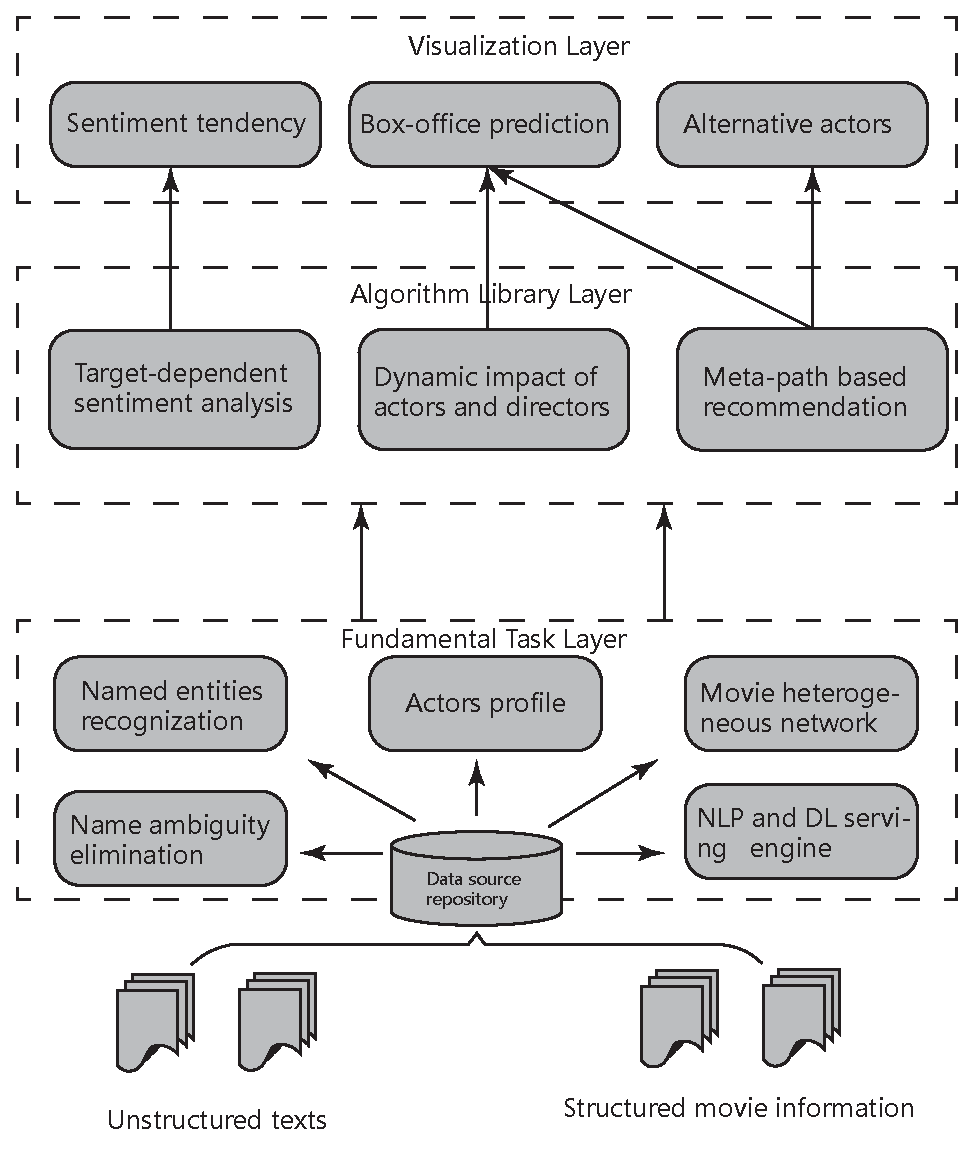
\includegraphics[width=0.8\columnwidth]{overview.eps}
\caption{System architecture}
\label{fig:arch}
\end{figure}

\begin{figure*}[!htbp]
  \centering
     \subfloat[dashboard]{%
  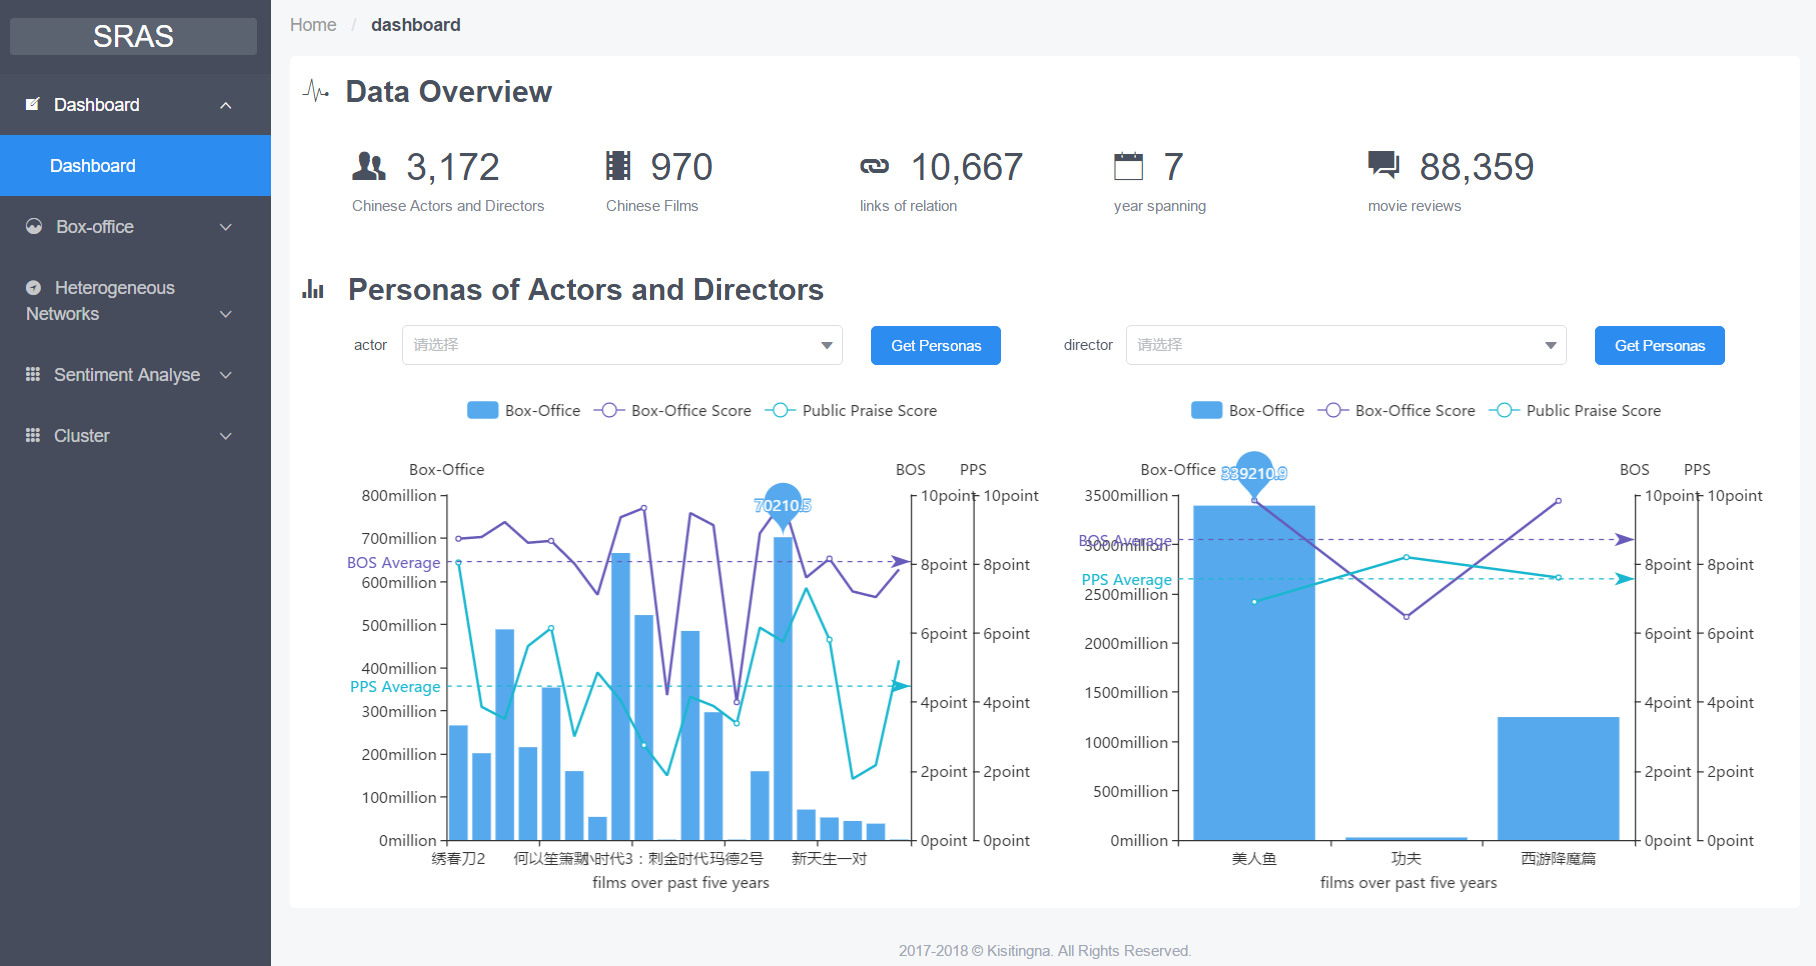
\includegraphics[width=0.32\linewidth]{screenshot_dashboard.png}}\hfill
      \subfloat[film level sentiment]{%
  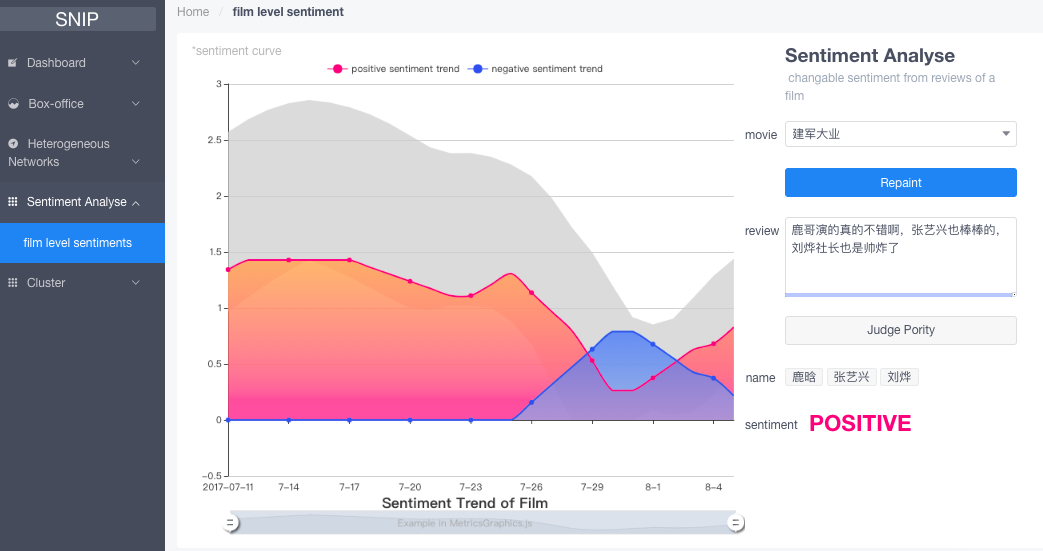
\includegraphics[width=0.32\linewidth]{screenshot_senti.png}}\hfill
      \subfloat[hierarchical cluster]{%
  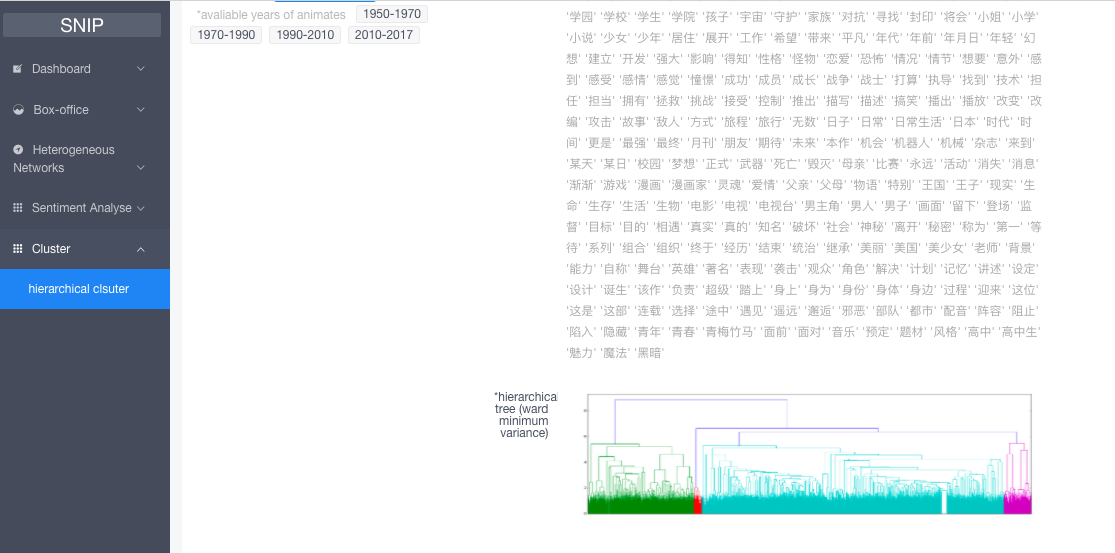
\includegraphics[width=0.32\linewidth]{screenshot_text.png}}\hfill
    \subfloat[dynamic impact]{%
  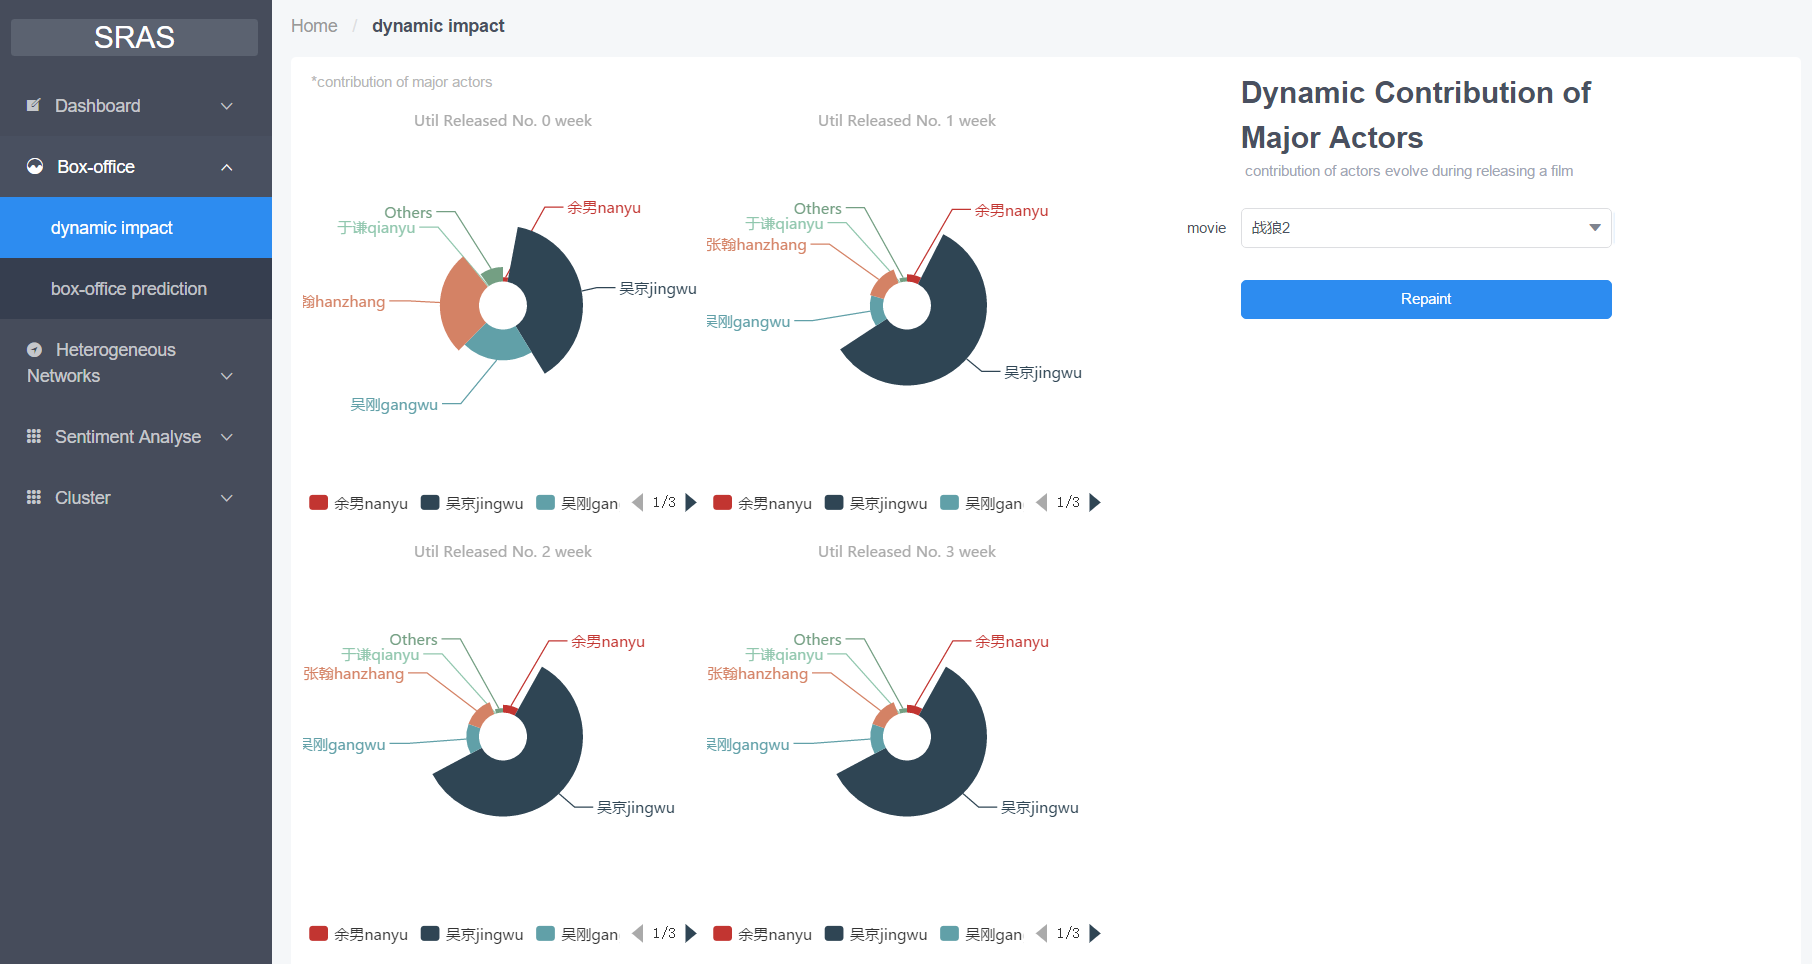
\includegraphics[width=0.32\linewidth]{screenshot_dynamic.png}}\hfill
    \subfloat[phased box-office prediction]{%
  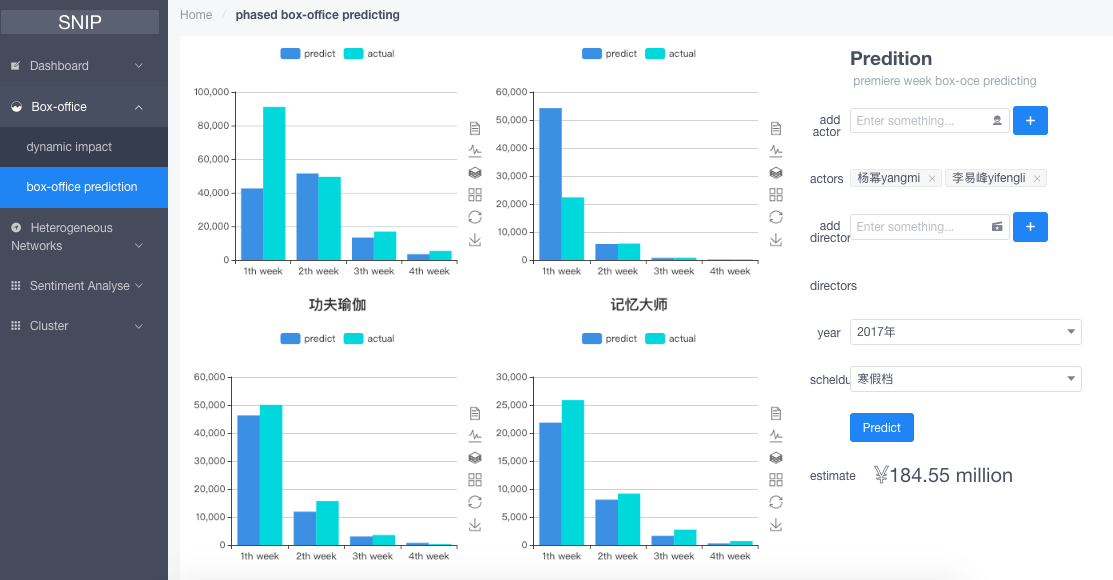
\includegraphics[width=0.32\linewidth]{screenshot_predict.png}}\hfill
    \subfloat[heterogeneous network]{%
  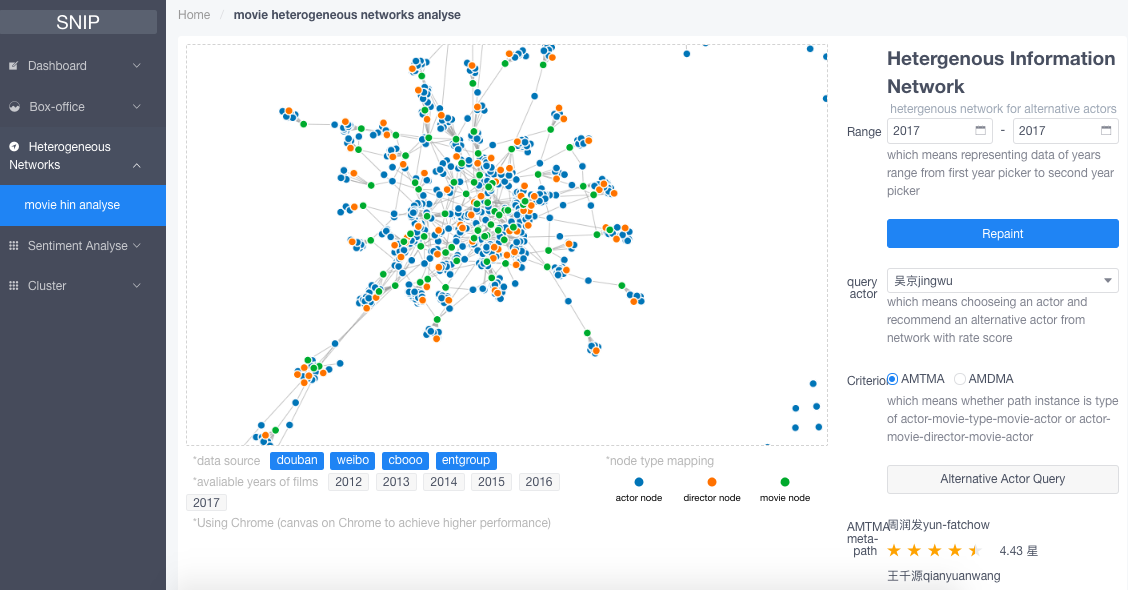
\includegraphics[width=0.32\linewidth]{screenshot_network.png}}\hfill
  \caption{Screenshots of \system}
  \label{fig:screen}
\end{figure*}



\system is a web-based integrated system for movie analysis. The architecture overview is displayed in Figure \ref{fig:arch}. Using \system, users can carry out a series of analysis based on the movie centric information.
\par In general, \system consists of three layers of components, including Basic Processing Task Layer, Higher Algorithm Library Layer and Visualization Layer.
\par Basic Processing Task Layers provides data cleaning, data standardization and data conversion. Due to the different data sources, the data obtained can not be applied directly to the analysis. In fact, the movie data need to consider the following questions, name ambiguity elimination, used to evaluate the quality of the film at the box office, the film's reviews of object identification, actor knowledge base construction. These methods are provided in the basic processing task layer.
\par Higer Algorithm Library Layer contains the core technology of \system, including Target-Dependent Sentiment Analysis Module and Dynamic Impact of Actors and Directors Module. The layer considers the importance of film reviews to a film and combine with Machine Learning.
\par Visualization Layer is the interface between the system and the users. To intuitively present the analysis results, this layer is designed to be user-friendly and easy to operate. Specifically, Sentiment Tendency is to capture the changes of sentiment among audience during movie released. Box-office prediction is to predict the box office of a movie by actors, directors and audience factors. Alternative actors is to get the replaceable list of actors.
\par The screenshots of \system are shown in Figure \ref{fig:screen}. \ref{fig:screen}(a) records messages we obtained and descriptions about all actors and directors. \ref{fig:screen}(b) and \ref{fig:screen}(c) are both related to Section \ref{sec:sent}. \ref{fig:screen}(b) can illustrate the change of sentiment trend about a cast in a movie but \ref{fig:screen}(c) illustrates the change of that during a movie releases and we provide a function that users enter a sentence and a movie, they can obtain cast with positive or negtive sentiment. \ref{fig:screen}(d) is a screenshot that captures dynamic influences  of cast and directors in a movie. \ref{fig:screen}(e) provides a box-office predicting module. Both \ref{fig:screen}(d) and \ref{fig:screen}(e) are related to Section \ref{sec:impact}. \ref{fig:screen}(f) related to Section \ref{sec:hin} provides a interface of actor recommendation based on actors network we construct.

